\section{Financial models of communication}

Late to a meeting is theft, and poorly written email and email to the wrong people has financial cost.

\subsection*{Meeting time compared to theft}
% https://graphthinking.blogspot.com/2021/02/organizations-value-things-more-than.html

In large organizations, there can be significant bureaucracy associated with even small purchases. A multi-step review process may be incurred for a \$2000 acquisition.

Another measurement of value is that if an employee were to steal even \$200 worth of materials, the organization would likely punish that employee.


In the book High Output Management~\cite{1995_Grove}, Grove points out that those metrics apply to tangible goods, but not to people's time. Consider a meeting of 10 people and each person's cost is \$200 per hour. 
\marginpar{[Tag] Math}
A wasted meeting is not unusual and certainly would not incur bureaucratic review processes. The cost to the organization is fiscally the same -- \$2000. Similarly, consider an employee who is late and causes a loss of productivity. Merely depriving the organization of \$200 worth of time is not punished in the same way theft is.

In fact, organizations default to meetings (even recurring meetings) rather than not meet. And being late to a meeting is accepted. 

We can debate the differences between theft of materials and theft of time. The financial argument is clear. 


\subsection*{Email is not free}

Total cost of email:
\begin{itemize}
    \item time spent writing
    \item time spent reading
    \item infrastructure maintenance
\end{itemize}

\marginpar{[Tag] Math}
\begin{multline}
\text{Cost per email} = 
(\text{hourly rate of writer})*(\text{time spent writing}) +\\
(\text{hourly rate of reader})*(\text{time spent reading})*(\text{number of readers})+\\
\frac{\text{annual salary of maintainer}}{\text{number of emails per year}} + \frac{\text{email server cost}}{\text{number of emails per year}}
\end{multline}
Plugging in some numbers, suppose an author charging \$50 per hour spends 5 minutes writing an email to 4 people. Each of those four people also charge \$50 per hour and spends 5 minutes on reading. 
\begin{equation}
50*(5/60) + 50*(5/60)*4 + \frac{100000}{1000000} + \frac{10000}{1000000} = \$21
\label{eq:four_readers}
\end{equation}
for one email!

\begin{figure}
    \centering
    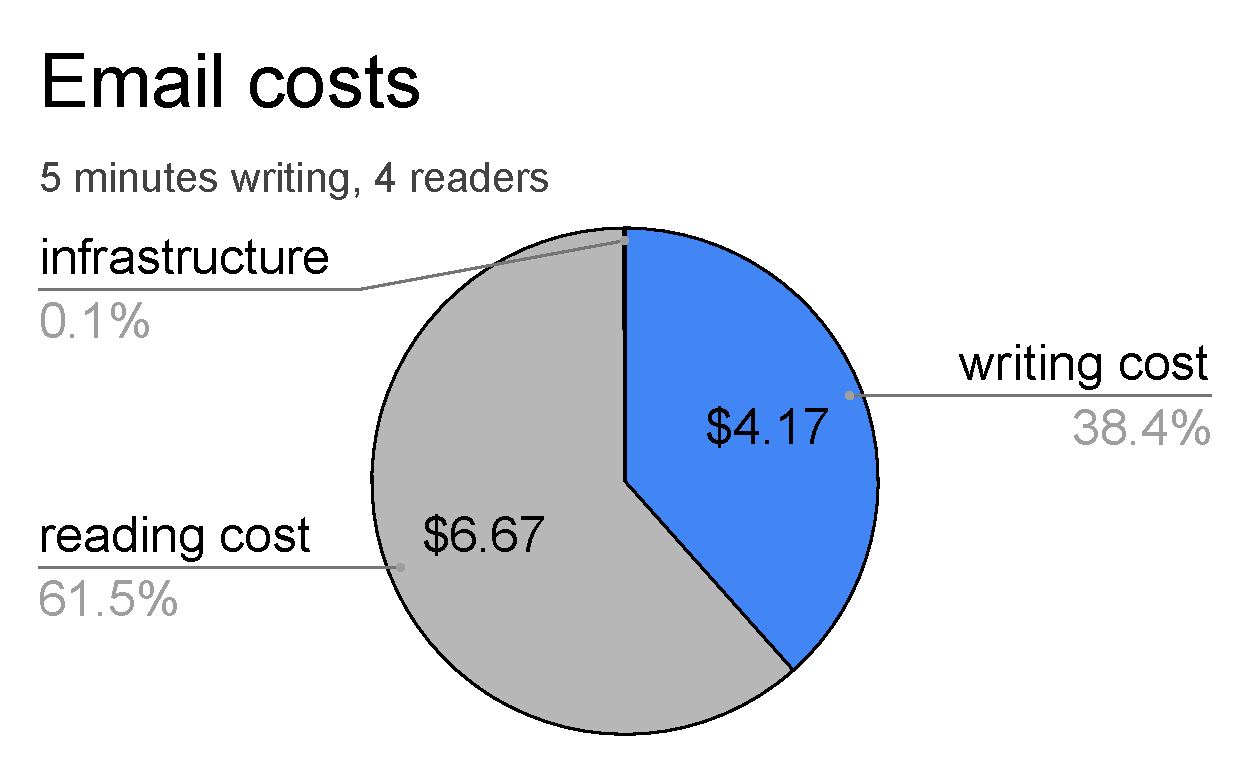
\includegraphics[width=0.7\textwidth]{images/email_costs_5minutes_4people.pdf}
    \caption{Breakdown of costs for Equation~\ref{eq:four_readers}. If \$21 for an email doesn't seem too significant, consider the broader releavnce to the organization. If email consumes 2 hours a day per person, and staffing is 50\% of the organizations budget, then 
    % (2/8)*0.5
    12.5\% of the organization's budget is spent on email. The same math for applies to meetings, so that's 25\% of the organization's budget on coordination.}
    \label{fig:my_label}
\end{figure}

% https://docs.google.com/spreadsheets/d/1ysV5PA3cEcneKv5BViUhAfgNq26cOlNRj6l5fXuHM3Q/edit?usp=sharing


%Paradigm for reading emails
%* Unread
%* Does this message have any bearing on my current task? 
%* Integrate with my understanding 